\section{LongMemEval-M: an exploratory controller-only run}
\label{sec:lme}
\subsection{Setup}
We ran the scorecard controller of Section~\ref{sec:interface} on a 180-question slice of LongMemEval-M \citep{arxiv_2410_10813}, stratified at 30 questions for each of the six question types (knowledge update, multi-session, single-session assistant, single-session preference, single-session user, temporal reasoning). The answer model was \texttt{qwen/qwen3.5-9b} with reasoning disabled, the judge was \texttt{google/gemma-4-31b-it}, and candidates were extracted turn by turn from the question's sessions into a fresh in-memory store for each question. The run used eight shards and three invocations recorded in its manifest; 28 worker processes stopped abnormally (25 runtime errors and 3 interruptions), and the manifest records an exit code of 1 and a status that was never changed from ``running''. According to the run manifest, which records one control set, and the study owner, the execution was interrupted and subsequently resumed under the same frozen controls rather than treated as a new experimental condition; per-invocation control hashes were not recorded. Result coverage was checked after the run: each of the 180 expected question identifiers (the set attested by the manifest) occurs exactly once in the predictions, answers and judgments, from exactly one shard, with no missing, duplicate or unexpected identifier. Operational metadata of the last invocation are incomplete. The completed outputs were merged from the shards (Appendix~\ref{app:prov} describes how the run directory and the code were verified). The answer provider policy allowed fallback among three providers, and the provider that served each call was not reported. The slice had informed the development of the controller: the analysis plan frozen before the run states that the V12 implementation was selected after inspecting partial V11 outcomes on this slice, and that for this reason the tests, intervals and acceptance readout from this run are descriptive and exploratory. The run's acceptance target of 153 of 180 correct answers was not met.

\subsection{Results}
The grader scored 128 of 180 answers as correct (0.711): 118 by parsed verdicts of the model judge, 8 by deterministic guards applied before the judge (40 of the 180 answers were never sent to the judge, and 32 of those were scored incorrect), and 2 by a substring fallback after unparseable judge output. After nine manual adjudications described below, the count was 137 of 180 (0.761). Table~\ref{tab:lme} gives both counts by question type. Exact (Clopper--Pearson) 95\% intervals are 0.639 to 0.776 for 128 of 180 and 0.692 to 0.821 for 137 of 180. The post-adjudication report records eight correct answers among the nine abstention questions. The results are for one run. A request seed of 0 was sent to the hosted answer model, but whether the provider honors it is unknown, so determinism of the answers is not established.

\begin{table}[t]
\centering\small
\caption{Controller-only V12 run on 180 LongMemEval-M questions: correct answers by question type on the grader's output, and after nine manual adjudications (30 questions per type).}
\label{tab:lme}
\begin{tabular}{lcc}
\toprule
Question type & Grader output & After adjudication \\
\midrule
Knowledge update & 29 & 29 \\
Multi-session & 19 & 19 \\
Single-session assistant & 29 & 29 \\
Single-session preference & 9 & 16 \\
Single-session user & 24 & 25 \\
Temporal reasoning & 18 & 19 \\
\midrule
Total (of 180) & 128 & 137 \\
\bottomrule
\end{tabular}
\end{table}

\paragraph{The nine adjudications.} Nine judgments were changed by hand from incorrect to correct. All nine concern the controller's outputs, none changed in the other direction, and seven fall in the single-session-preference type (Figure~\ref{fig:lme}). Eight of the nine changed a verdict of the model judge and one changed a verdict from a deterministic guard. The nine identifiers are a hard-coded list in three scripts, each with a short written reason, and the original judge output is kept in backup files. According to the study owner, the nine cases were adjudicated by an independent human reviewer. The available artifacts record neither the reviewer identity nor the review date, and no file records why these nine were chosen or how many of the 52 failures of the controller were reviewed. The same procedure was not applied to the baselines. According to the study owner, their three overrides came from a separate pass by an independent human reviewer. The available artifacts record no reviewer identity, review date or tool, and do not record the selection criteria or review coverage for that pass. The frozen analysis plan asks that results be reported on the raw judge score first and that any adjudication be reported as a separate sensitivity analysis; we therefore treat 128 of 180 as the primary count and 137 of 180 as a one-sided post-hoc sensitivity count, which should not be read as an independently adjudicated accuracy. Seven of the nine reviewed cases were in the preference type; how the cases were selected and how many other failures were examined are not documented, so we draw no conclusion about where the model judge and a human reader disagree.

\begin{figure}[t]
\centering
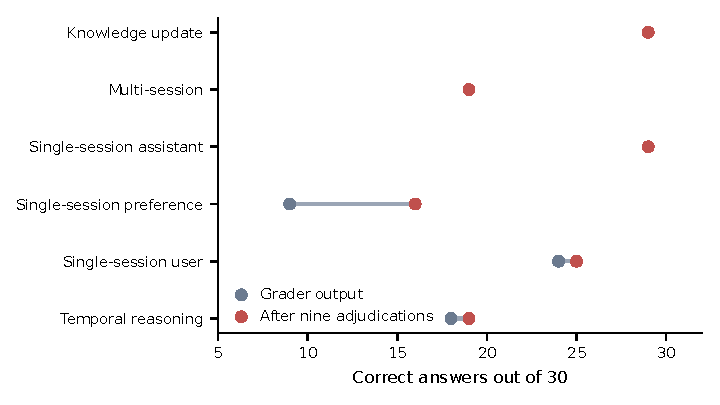
\includegraphics[width=0.78\linewidth]{figures/fig_lme.pdf}
\caption{Correct answers out of 30 by question type for the V12 controller-only run, on the grader's output and after the nine manual adjudications.}
\label{fig:lme}
\end{figure}

\paragraph{Why no comparison with other systems is reported.} The run directory contains judgments for four baselines (no memory, flat retrieval, recency, naive overwrite). They are byte-identical to the baselines of an earlier run that used a different freeze version, a different shard layout and a different judge configuration (the earlier manifest names a free-tier primary judge with a fallback, whereas its call logs record requests to the identifier without the free-tier suffix, routed to a dated revision), and the model identifiers recorded for the baselines differ in form from those of the controller (a dated slug versus an undated identifier). The V12 run itself evaluated only the controller; its run matrix says that it does not support comparative claims and defines a separate five-system run for that purpose. Three baseline judgments (one for the no-memory baseline, two for naive overwrite) carry override fields. The repository's failure ledger describes comparable manual overrides in an earlier run (v7), made in place and without an executable manifest; it does not document these three. According to the study owner, the three overrides were made by an independent human reviewer. Originals were kept in backup files, but the reviewer identity, date and criteria are not recorded in the available artifacts, and we did not find the tool that wrote them. The plan requires a homogeneity check (one configuration and one judge policy for all systems) before comparative claims. The check as recorded in the run directory returned false because of a stale launcher hash, and it covered the controller only; we found no record of the five-system check required by the plan, and the baseline heterogeneity described above was identified separately. We do not report paired tests between the controller and the baselines. Appendix~\ref{app:baselines} lists the baseline counts as context only.

\subsection{Decision log and replay}
The merged action log of the run holds 12\,654 decisions from 3\,547 sessions. Of these rows, 11\,832 were written by the worker that completed each question and 822 (6.5 percent) are rows of 20 partial question runs that stopped and were replayed after a restart; the log is opened in append mode on resume and the merge step does not deduplicate it. The completed question runs contain 10\,712 \keep{} (0.905), 373 \supersede{} (0.032) and 747 \abstain{} (0.063) decisions, over 9\,192 episodic facts, 2\,273 transient preferences and 367 stable preferences; the 822 stale rows add 766, 24 and 32 respectively (all 12\,654 rows: 11\,478, 397 and 779). All supersessions carry a predecessor and a successor identifier, and no abstention row carries a resulting identifier. Most \keep{} rows of the merged log (10\,778 of 11\,478) have no compared prior. Of the 10\,712 \keep{} rows of the completed runs, 10\,699 carry a resulting memory identifier, that is, the candidate was inserted as a new active record; in this runtime \keep{} means a non-superseding acceptance of the candidate and almost never a withheld write (Section~\ref{sec:interface}). Action statistics taken from the merged log include the stale rows unless they are excluded; the exclusion list is in the supplement.

We recomputed the scorecard decision for every one of the 12\,654 rows from its logged features, with the scorecard code of the released commit and its default configuration. All actions matched, and the recomputed scores and thresholds matched the logged values with a maximum absolute deviation of 0.0. This establishes replay level R1 (decision-rule replay) for this log, which we bind to the log's SHA-256 hash. R1 shows deterministic recomputation conditional on the logged feature rows; stale rows are themselves outputs of the rule, so R1 holds for them too, and it does not establish that every logged row corresponds one-to-one to an intended extraction event. It also does not establish that the features were extracted correctly, that the store reached the intended state, or that retrieval and answer generation are reproducible; those levels (R2 to R7, Appendix~\ref{app:replay}) are not established. The scorecard modules are not among the files whose hashes the run manifest recorded, so the exact match shows that the released scorecard gives the same decisions and scores on all 12\,654 logged feature vectors; we cannot show that the hosted language models would return the same features again.

The extraction trace and cache hold 11\,771 validated extracted items, while the merged log holds 883 more decisions than items. The two counts are in different units. In comparable units, 12\,654 = 11\,832 + 822 and 11\,832 = 11\,771 + 61. The 822 rows are the stale rows above: each of the 20 stale groups equals, in order, the leading rows of the same question as re-run by the completing worker (822 of 822 rows). The 61 rows are repeated decisions on one cached extraction output that the same shard reuses for two or more questions. The allocation, which rests on stated assumptions about the log and the shard progress files, leaves no row of the 883 unexplained; one extraction-trace row without a cache entry and 16 of 43 repeated cache lookups cannot be characterised at item level, and 23 rows have a cache item whose recorded evidence session differs from the session in which the candidate was ingested.
